\documentclass[12pt,letterpaper]{article}
\usepackage{fullpage}
% Margins
\usepackage[top=2cm, bottom=4.5cm, left=2.5cm, right=2.5cm]{geometry}
\usepackage{amsmath,amsthm,amsfonts,amssymb,amscd}
\usepackage{lastpage}
\usepackage{enumerate}
\usepackage{fancyhdr}
\usepackage{mathrsfs}
\usepackage{xcolor}
\usepackage{graphicx}
\usepackage{listings}
\usepackage{hyperref}
\usepackage{txfonts}
\usepackage{titlesec}

% For hyperlinks if I ever use them
\hypersetup{%
	colorlinks=true,
	linkcolor=blue,
	linkbordercolor={0 0 1}
}

% Edit these every document
\newcommand\course{CS 2200}
\newcommand\hwnumber{5}                 
\newcommand\Name{Owen Miller-Fast}
\newcommand\email{ormd3n@umsystem.edu}

% \renewcommand\lstlistingname{Algorithm}
% \renewcommand\lstlistlistingname{Algorithms}
% \def\lstlistingautorefname{Alg.}

% Subsections use letters instead of numbers
\renewcommand{\thesubsection}{\thesection.\alph{subsection}}

\setlength{\parindent}{0.0in}
\setlength{\parskip}{0.05in}

% Formatting sections and subsections
\titleformat{\section}{\normalfont\bfseries}{Problem \thesection:}{1em}{}
\titleformat{\subsection}{\normalfont\bfseries}{\thesubsection)}{2em}{}
\fancypagestyle{firstpage}
{
	\lhead{\Name{}\\\email}
	\chead{\textbf{Homework \hwnumber}}
	\rhead{\course\\\today}
}
\fancypagestyle{following}
{
	\lhead{\Name{}\\\email}
	\rhead{\course\\\today}
}

\pagestyle{fancyplain}
\thispagestyle{firstpage}
\pagestyle{following}
\headheight 35pt
% Footer
\lfoot{}
\cfoot{}
\rfoot{\small\thepage}
\headsep 1em

\begin{document}
	\section{CFG Creation}
		Let the following terminals represent characters:
		\begin{itemize}
			\item \textit{a} = (
			\item \textit{b} = )
			\item \textit{c} = \{
			\item \textit{d} = \}
			\item \textit{e} = [
			\item \textit{f} = ]
		\end{itemize}
		The following machine, $G_1$, generates all possible correcting nesting of parenthesis, braces, and brackets:\\
		
		$V=\{S\}\\\sum=\{a,b,c,d,e,f\}\\$
		$R:$
		\begin{gather*}
			S \rightarrow SS\arrowvert aSb\arrowvert cSd\arrowvert eSf\arrowvert \varepsilon
		\end{gather*}
		$S\in V=S$\\
		$G_1=(V,\sum,R,S)$
	\section{CFG Conversion}
		\textit{Start variable}: \textit{S}\\
		
		\textbf{Step 1: Add new start variable}
		\begin{gather*}
			\textcolor{green}{S_1\rightarrow S}\\
			S \rightarrow SS\arrowvert aSb\arrowvert cSd\arrowvert eSf\arrowvert \varepsilon
		\end{gather*}
		\textbf{Step 2: Eliminate $\varepsilon$-rules}
		\begin{gather*}
			S_1\rightarrow S\\
			S \rightarrow SS\arrowvert aSb\arrowvert cSd\arrowvert eSf\arrowvert \textcolor{blue}{\varepsilon}\\
			\\S_1\rightarrow S\arrowvert \textcolor{green}{\varepsilon}\\
			S \rightarrow SS\arrowvert aSb\arrowvert cSd\arrowvert eSf\arrowvert \textcolor{green}{ab}\arrowvert \textcolor{green}{cd}\arrowvert \textcolor{green}{ef}
		\end{gather*}
		\textbf{Step 3: Remove unit rules}\\
		\\Step 3a: Removing $S_1\rightarrow S$
		\begin{gather*}
			S_1\rightarrow \textcolor{blue}{S}\arrowvert \varepsilon\\
			S \rightarrow SS\arrowvert aSb\arrowvert cSd\arrowvert eSf\arrowvert ab\arrowvert cd\arrowvert ef\\
			\\S_1\rightarrow \varepsilon\arrowvert \textcolor{green}{SS}\arrowvert \textcolor{green}{aSb}\arrowvert \textcolor{green}{cSd}\arrowvert \textcolor{green}{eSf}\arrowvert \textcolor{green}{ab}\arrowvert \textcolor{green}{cd}\arrowvert \textcolor{green}{ef}\\
			S \rightarrow SS\arrowvert aSb\arrowvert cSd\arrowvert eSf\arrowvert ab\arrowvert cd\arrowvert ef
		\end{gather*}
		\\Step 3b: Adding $Z_1-Z_9$
		\begin{gather*}
			S_1\rightarrow \varepsilon\arrowvert SS\arrowvert aSb\arrowvert cSd\arrowvert eSf\arrowvert ab\arrowvert cd\arrowvert ef\\
			S \rightarrow SS\arrowvert aSb\arrowvert cSd\arrowvert eSf\arrowvert ab\arrowvert cd\arrowvert ef\\
			\\S_1\rightarrow \varepsilon\arrowvert SS\arrowvert aSb\arrowvert cSd\arrowvert eSf\arrowvert ab\arrowvert cd\arrowvert ef\\
			S \rightarrow SS\arrowvert aSb\arrowvert cSd\arrowvert eSf\arrowvert ab\arrowvert cd\arrowvert ef\\
			\textcolor{green}{Z_1\rightarrow SZ_5}\\
			\textcolor{green}{Z_2\rightarrow SZ_7}\\
			\textcolor{green}{Z_3\rightarrow SZ_9}\\
			\textcolor{green}{Z_4\rightarrow a}\\
			\textcolor{green}{Z_5\rightarrow b}\\
			\textcolor{green}{Z_6\rightarrow c}\\
			\textcolor{green}{Z_7\rightarrow d}\\
			\textcolor{green}{Z_8\rightarrow e}\\
			\textcolor{green}{Z_9\rightarrow f}\\
		\end{gather*}
		\textbf{Step 4: Fix rules}
		\begin{gather*}
			S_1\rightarrow \varepsilon\arrowvert SS\arrowvert \textcolor{blue}{aSb}\arrowvert\textcolor{blue}{cSd}\arrowvert \textcolor{blue}{eSf}\arrowvert\textcolor{blue}{ab}\arrowvert \textcolor{blue}{cd}\arrowvert\textcolor{blue}{ef}\\
			S \rightarrow SS\arrowvert \textcolor{blue}{aSb}\arrowvert \textcolor{blue}{cSd}\arrowvert \textcolor{blue}{eSf}\arrowvert 	\textcolor{blue}{ab}\arrowvert \textcolor{blue}{cd}\arrowvert \textcolor{blue}{ef}\\
			Z_1\rightarrow SZ_5\\
			Z_2\rightarrow SZ_7\\
			Z_3\rightarrow SZ_9\\
			Z_4\rightarrow a\\
			Z_5\rightarrow b\\
			Z_6\rightarrow c\\
			Z_7\rightarrow d\\
			Z_8\rightarrow e\\
			Z_9\rightarrow f\\
			\\S_1\rightarrow \varepsilon\arrowvert SS\arrowvert \textcolor{green}{Z_4Z_1}\arrowvert \textcolor{green}{Z_6Z_2}\arrowvert \textcolor{green}{Z_8Z_3}\arrowvert \textcolor{green}{Z_4Z_5}\arrowvert \textcolor{green}{Z_6Z_7}\arrowvert \textcolor{green}{Z_8Z_9}\\
			S\rightarrow SS\arrowvert \textcolor{green}{Z_4Z_1}\arrowvert \textcolor{green}{Z_6Z_2}\arrowvert \textcolor{green}{Z_8Z_3}\arrowvert \textcolor{green}{Z_4Z_5}\arrowvert \textcolor{green}{Z_6Z_7}\arrowvert \textcolor{green}{Z_8Z_9}\\
			Z_1\rightarrow SZ_5\\
			Z_2\rightarrow SZ_7\\
			Z_3\rightarrow SZ_9\\
			Z_4\rightarrow a\\
			Z_5\rightarrow b\\
			Z_6\rightarrow c\\
			Z_7\rightarrow d\\
			Z_8\rightarrow e\\
			Z_9\rightarrow f\\
		\end{gather*}
		\textbf{Answer}
		\begin{gather*}
			S_1\rightarrow \varepsilon\arrowvert SS\arrowvert Z_4Z_1\arrowvert Z_6Z_2\arrowvert Z_8Z_3\arrowvert Z_4Z_5\arrowvert Z_6Z_7\arrowvert Z_8Z_9\\
			S\rightarrow SS\arrowvert Z_4Z_1\arrowvert Z_6Z_2\arrowvert Z_8Z_3\arrowvert Z_4Z_5\arrowvert Z_6Z_7\arrowvert Z_8Z_9\\
			Z_1\rightarrow SZ_5\\
			Z_2\rightarrow SZ_7\\
			Z_3\rightarrow SZ_9\\
			Z_4\rightarrow a\\
			Z_5\rightarrow b\\
			Z_6\rightarrow c\\
			Z_7\rightarrow d\\
			Z_8\rightarrow e\\
			Z_9\rightarrow f\\
		\end{gather*}
	\section{Convert CFG to PDA}
	\begin{figure}[h!]
		\centering
		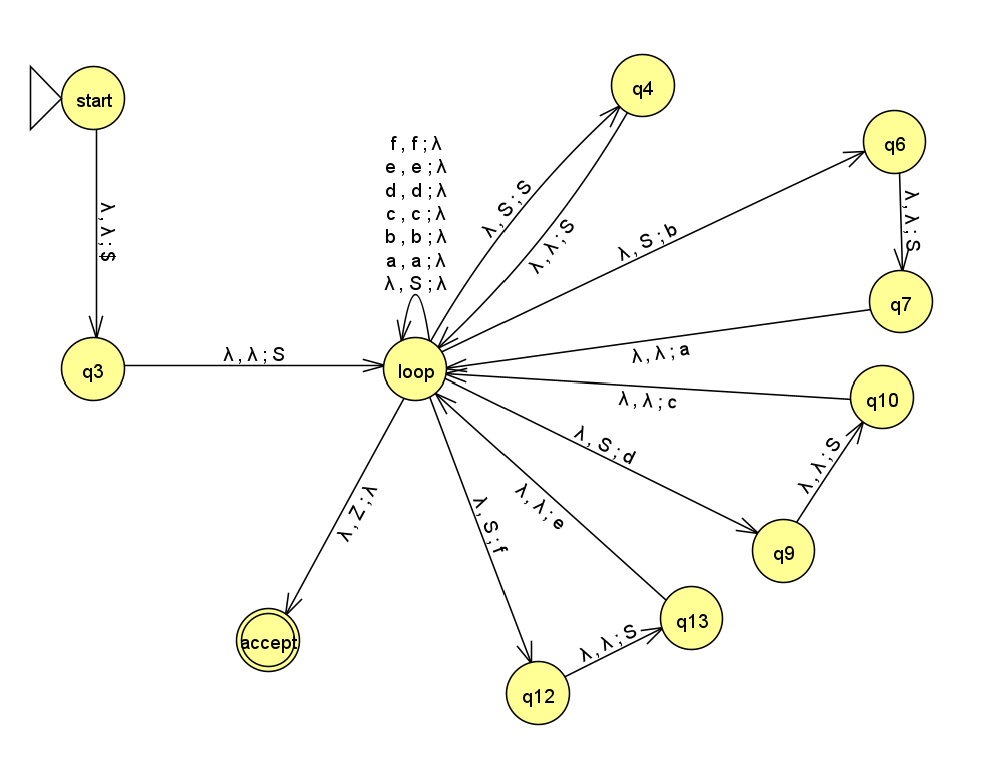
\includegraphics[width=0.8\textwidth]{pda.png}
	\end{figure}
\end{document}
